%\VignetteIndexEntry{Simulation visualization and plotting in SpaDES}
%\VignetteDepends{SpaDES}
%\VignetteKeyword{maps}
%\VignetteKeyword{plot}
%\VignetteKeyword{visualization}
\documentclass{article}

%%% latex packages
\usepackage{hyperref}
\usepackage[utf8]{inputenc}
\usepackage[usenames,dvipsnames]{xcolor}

%% change margins to 1" all the way around
\oddsidemargin 0.0in
\evensidemargin 0.0in
\textwidth 6.5in
\headheight 0.0in
\topmargin 0.0in
\textheight 9.0in

%%% document info
\title{Plotting with \texttt{Plot} in \texttt{SpaDES}}

\author{
  Eliot McIntire\\
	\small{Natural Resources Canada, Pacific Forestry Centre}\\
	\small{email: \href{mailto:emcintir@nrcan.gc.ca}{emcintir@nrcan.gc.ca}}
  \and
  Alex M. Chubaty\\
  \small{Natural Resources Canada, Pacific Forestry Centre}\\
  \small{email: \href{mailto:achubaty@nrcan.gc.ca}{achubaty@nrcan.gc.ca}}
}

\usepackage{Sweave}
\begin{document}
\Sconcordance{concordance:plotting.tex:plotting.Rnw:%
1 31 1 1 0 15 1}

 % displays code as entered (no arranging lines)

\maketitle

\tableofcontents

\newpage

\section{Plotting in \texttt{SpaDES}}

\paragraph{}
One of the major features of the \texttt{SpaDES} package is that can take advantage of the numerous visualization tools available natively or through user built packages (e.g., RgoogleVis, ggplo2, rgl). The main set of plotting functions that we have packaged with spades are built on top of the grid package. These allow for relatively fast plotting of rasters and points with the ability to make multi-frame plots without the module (or user) knowing which plots are already plotted. In other words, the main plotting function can handle modules that add plots, without them knowing what the current state of the active plotting device is. This means that the plotting can be also treated as modular.  Furthermore, conventional R plotting still works, so you can use the features provided in this package or you can use base plotting functions without having to relearn a completely new set of plotting commands. This is called with the workhorse function, \texttt{Plot}, i.e., capital P.

\section{The \texttt{Plot} function}
\paragraph{Layer types}
There are several features of Plot that are worth highlighting. First, it can plot a mixture of RasterLayers, RasterStacks and SpatialPoints* objects. In the code snippet below, we create the list of files to load, which is every file in the "maps" subdirectory of the package. Then we load that list of files. Because we specified .stackName in the fileList, the loadFiles function will automatically put the individual layers into a RasterStack; the individual layers will not be available as objects within the R environment. If .stackNames did not exist, then the individual files would be individual objects.

\paragraph{Names}
It is critical in SpaDES plotting that every layer has a \texttt{name}. This can be added to RasterLayers, RasterStacks or SpatialPoints objects using the assignment function in the form \texttt{name(Layer)<-"something"}.

\paragraph{Colors}
Every Raster can have a colortable, which gives the mapping of raster values to colors. If not already set in the file (many .tif files already have their colortable set), we can use setColors(Raster*) with a named list of hex colours, if a RasterStack, or just a vector of hex colors if only a single RasterLayer. These can be easily built with the RColorBrewer package, with the function brewer.pal().

\paragraph{add}
The argument \texttt{add} can add plots to

\paragraph{addTo}
The argument addTo will allow overplotting of

Below, we see file loading, naming, setting colors and plotting.
\begin{Schunk}
\begin{Sinput}
> #  Make list of maps from package database to load, and what functions to use to load them
> library(SpaDES)
> fileList <-
+     data.frame(files =
+      dir(file.path(
+                    find.package("SpaDES",
+                                 lib.loc=getOption("devtools.path"),
+                                 quiet=FALSE),
+                   "maps"),
+         full.names=TRUE, pattern= "tif"),
+      functions="rasterToMemory",
+      .stackName="landscape",
+      packages="SpaDES",
+      stringsAsFactors=FALSE)
> #'
> # Load files to memory (using rasterToMemory) and stack them (because .stackName is provided above)
> loadFiles(fileList=fileList)
> #'
> # extract a single one of these rasters
> DEM <- landscape$DEM
> #'
> # can change color palette
> setColors(landscape, n = 50)<-list(DEM=topo.colors(50),
+                            forestCover = RColorBrewer::brewer.pal(9,"Set1"),
+                            forestAge = RColorBrewer::brewer.pal("Blues",n=8),
+                            habitatQuality = RColorBrewer::brewer.pal(9,"Spectral"),
+                            percentPine = RColorBrewer::brewer.pal("GnBu",n=8))
> #'
> #Make a new raster derived from a previous one; must give it a unique name
> habitatQuality2 <- landscape$habitatQuality ^ 0.3
> names(habitatQuality2) <- "habitatQuality2"
> #'
> # make a SpatialPointsNamed object
> caribou <- SpatialPointsNamed(coords=cbind(x=runif(1e2,-50,50),y=runif(1e2,-50,50)),
+                               name="caribou")
> #'
> #Plot all maps on a new plot windows - Do not use RStudio window
> #if(is.null(dev.list())) {
> #   dev(2)
> #} else {
>  # if(any(names(dev.list())=="RStudioGD")) {
>  #   dev(which(names(dev.list())=="RStudioGD")+3)
>  # } else {
>  #   dev(max(dev.list()))
>  # }
> #}
> #'
> Plot(landscape)
> #'
> # Can overplot, using addTo
> Plot(caribou, addTo="forestAge",size=4, axes=F)
> #'
> # can add a new plot to the plotting window
> Plot(caribou, add=T)
> #'
> # can mix stacks, rasters, SpatialPoint*Named
> Plot(landscape, habitatQuality2, caribou)
> #'
> # can mix stacks, rasters, SpatialPoint*Named
> Plot(landscape, caribou)
> Plot(habitatQuality2, add=T)
> 
\end{Sinput}
\end{Schunk}
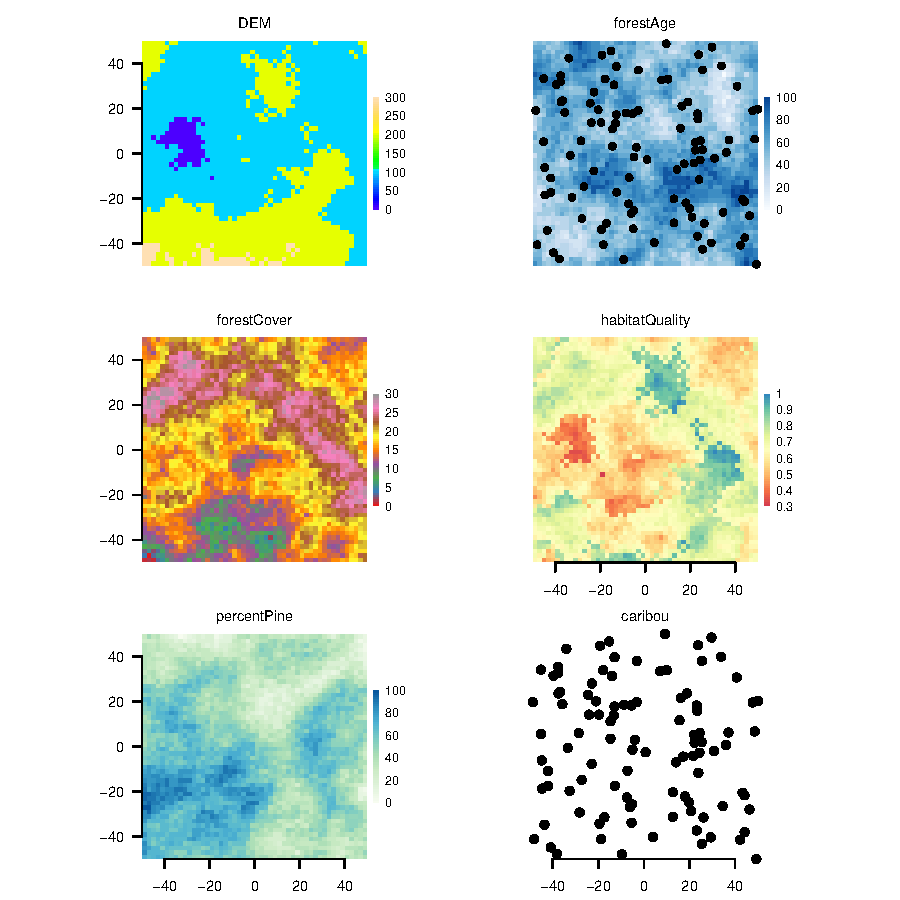
\includegraphics{plotting-plot-using-files}

\paragraph{}
There are several situations that do not plot. A call to Plot where there are two RasterLayers with the same name will return an error. This is true even if one of the layers is in a RasterStack, so is not explicitly called.
\begin{Schunk}
\begin{Sinput}
> Plot(landscape, caribou, DEM)
\end{Sinput}
\end{Schunk}
will return an error.

\end{document}

%
% %\VignetteIndexEntry{Simulation visualization and plotting in SpaDES}
% %\VignetteDepends{SpaDES}
% %\VignetteKeyword{maps}
% %\VignetteKeyword{plot}
% %\VignetteKeyword{visualization}
% \documentclass{article}
%
% %%% latex packages
% \usepackage{hyperref}
% \usepackage[utf8]{inputenc}
% \usepackage[usenames,dvipsnames]{xcolor}
%
% %% change margins to 1" all the way around
% \oddsidemargin 0.0in
% \evensidemargin 0.0in
% \textwidth 6.5in
% \headheight 0.0in
% \topmargin 0.0in
% \textheight 9.0in
%
% %%% document info
% \title{Plotting with \texttt{Plot} in \texttt{SpaDES}}
%
% \author{
%   Eliot McIntire\\
%   \small{Natural Resources Canada, Pacific Forestry Centre}\\
% 	\small{email: \href{mailto:emcintir@nrcan.gc.ca}{emcintir@nrcan.gc.ca}}
%   \and
%   Alex M. Chubaty\\
%   \small{Natural Resources Canada, Pacific Forestry Centre}\\
%   \small{email: \href{mailto:achubaty@nrcan.gc.ca}{achubaty@nrcan.gc.ca}}
% }
%
% \begin{document}
% \SweaveOpts{concordance=TRUE}
% \SweaveOpts{keep.source=TRUE} % displays code as entered (no arranging lines)
%
% \maketitle
%
% \tableofcontents
%
% \newpage
%
% \section{Plotting in \texttt{SpaDES}}
%
% \paragraph{}
% One of the major features of the \texttt{SpaDES} package is that can take advantage of the numerous visualization tools available natively or through user built packages (e.g., RgoogleVis, ggplo2, rgl). The main set of plotting functions that we have packaged with spades are built on top of the grid package. These allow for relatively fast plotting of rasters and points with the ability to make multi-frame plots without the module (or user) knowing which plots are already plotted. In other words, the main plotting function can handle modules that add plots, without them knowing what the current state of the active plotting device is. This means that the plotting can be also treated as modular.  Furthermore, conventional R plotting still works, so you can use the features provided in this package or you can use base plotting functions without having to relearn a completely new set of plotting commands. This is called with the workhorse function, \texttt{Plot}, i.e., capital P.
%
% \section{The \texttt{Plot} function}
%
% \paragraph{Layer types}
% There are several features of Plot that are worth highlighting. First, it can plot a mixture of RasterLayers, RasterStacks and SpatialPoints* objects. In the code snippet below, we create the list of files to load, which is every file in the "maps" subdirectory of the package. Then we load that list of files. Because we specified .stackName in the fileList, the loadFiles function will automatically put the individual layers into a RasterStack; the individual layers will not be available as objects within the R environment. If .stackNames did not exist, then the individual files would be individual objects.
%
% Below, we initiate with file loading.
% <<load-files, eval=TRUE, echo=TRUE, fig=TRUE, cache=TRUE>>=
% #  Make list of maps from package database to load, and what functions to use to load them
% library(SpaDES)
% fileList <-
%     data.frame(files =
%      dir(file.path(
%                    find.package("SpaDES",
%                                 lib.loc=getOption("devtools.path"),
%                                 quiet=FALSE),
%                   "maps"),
%         full.names=TRUE, pattern= "tif"),
%      functions="rasterToMemory",
%      #.stackName="landscape",
%      packages="SpaDES",
%      stringsAsFactors=FALSE)
% #'
% # Load files to memory (using rasterToMemory) and stack them (because .stackName is provided above)
% loadFiles(fileList=fileList)
% @
%
% \paragraph{Colors}
% Every Raster can have a colortable, which gives the mapping of raster values to colors. If not already set in the file (many .tif files already have their colortable set), we can use setColors(Raster*) with a named list of hex colours, if a RasterStack, or just a vector of hex colors if only a single RasterLayer. These can be easily built with the RColorBrewer package, with the function brewer.pal().
%
% <<colors, eval=TRUE, echo=TRUE, fig=FALSE, cache=TRUE>>=
% # extract a single one of these rasters
% # can change color palette
% setColors(landscape, n = 50)<-list(DEM=topo.colors(50),
%                            forestCover = RColorBrewer::brewer.pal(9,"Set1"),
%                            forestAge = RColorBrewer::brewer.pal("Blues",n=8),
%                            habitatQuality = RColorBrewer::brewer.pal(9,"Spectral"),
%                            percentPine = RColorBrewer::brewer.pal("GnBu",n=8))
% @
%
%
% \paragraph{Names}
% It is critical in SpaDES plotting that every layer has a \texttt{name}. This can be added to RasterLayers, RasterStacks or SpatialPoints objects using the assignment function in the form \texttt{name(Layer)<-"something"}. We can also use various extended builder functions, RasterStackNamed, SpatialPointsNamed, and SpatialPointsDataFrameNamed.
% <<naming, eval=TRUE, echo=TRUE, fig=FALSE, cache=TRUE>>=
% #Make a new raster derived from a previous one; must give it a unique name
% habitatQuality2 <- landscape$habitatQuality ^ 0.3
% names(habitatQuality2) <- "habitatQuality2"
%
% DEM <- landscape$DEM
% forestAge <- landscape$forestAge
% newLandscape <- RasterStackNamed(stack(DEM, forestAge), name="newLandscape")
% #'
% # make a SpatialPointsNamed object
% caribou <- SpatialPointsNamed(coords=cbind(x=runif(1e2,-50,50),y=runif(1e2,-50,50)),
%                               name="caribou")
% @
%
% \paragraph{add}
% The argument \texttt{add} can add RasterLayers, RasterStacks or SpatialPoints* in new plotting windows within the same active device. The function will do name matching, and so overplot any layer that was already previously plotted. Also, if there is not enough space on the current plot, it will re-arrange the plots to maintain an optimal visual arrangements.
%
% <<Plotting, eval=TRUE, echo=TRUE, fig=TRUE, cache=TRUE>>=
% Plot(landscape)
% Plot(caribou, add=T)
% @
%
%
% \paragraph{addTo}
% The argument addTo will allow overplotting of differently named layers. This may be useful for plotting SpatialPoint* objects or Raster* objects that have transparency.
%
% <<addTo, eval=TRUE, echo=TRUE, fig=TRUE, cache=TRUE>>=
% # Can overplot, using addTo
% Plot(landscape)
% Plot(caribou, addTo="forestAge",size=4, axes=F)
% @
%
% \paragraph{Arrangement of plots}
% The \texttt{Plot} function automatically optimally arranges all the named objects within the active device window. This means that it will minimize white space for any combination of plotted objects.
%
% <<mixing-types, eval=TRUE, echo=TRUE, fig=TRUE, cache=TRUE>>=
% # can mix stacks, rasters, SpatialPoint*Named
% Plot(landscape, habitatQuality2, caribou)
% #'
% # can mix stacks, rasters, SpatialPoint*Named
% Plot(landscape, caribou)
% Plot(habitatQuality2, add=T)
% @
%
% <<plot-fun, eval=TRUE, echo=TRUE, fig=TRUE>>=
% Plot(landscape)
% @
%
% \paragraph{}
% There are several situations that do not plot. A call to Plot where there are two RasterLayers with the same name will return an error. This is true even if one of the layers is in a RasterStack, so is not explicitly called.
% <<plot-errors, eval=FALSE, echo=TRUE>>=
% DEM <- landscape$DEM
% Plot(landscape, caribou, DEM)
% @
% will return an error.
%
% #Plot all maps on a new plot windows - Do not use RStudio window
% #if(is.null(dev.list())) {
% #   dev(2)
% #} else {
%  # if(any(names(dev.list())=="RStudioGD")) {
%  #   dev(which(names(dev.list())=="RStudioGD")+3)
%  # } else {
%  #   dev(max(dev.list()))
%  # }
% #}
%
%
% \end{document}
%
